\documentclass{article}
\usepackage{graphicx}
\usepackage{siunitx}

% prompted chatGPT to help me display figures in a 2x2 grid as opposed to vertically
% response helped me include these packages and display the figure
\usepackage{caption}       
\usepackage{subcaption}

\begin{document}

\section*{Implementation}
The implementation went smoothly, largely due to my prior experience with Python. I used ChatGPT several times for help, specifically with plotting. It served as a useful reference, effectively providing documentation by explaining the options available and how they worked. This approach worked well because I wasn't always sure what I needed to do, and being able to see all possible options was helpful.

\section*{Questions}
\subsection*{1.}
all figures have a width of 14 and height of 6

% LLM output:
\begin{figure}[h]
    \centering
    % First Subfigure (Top Left)
    \begin{subfigure}[t]{0.45\textwidth}
        \centering
        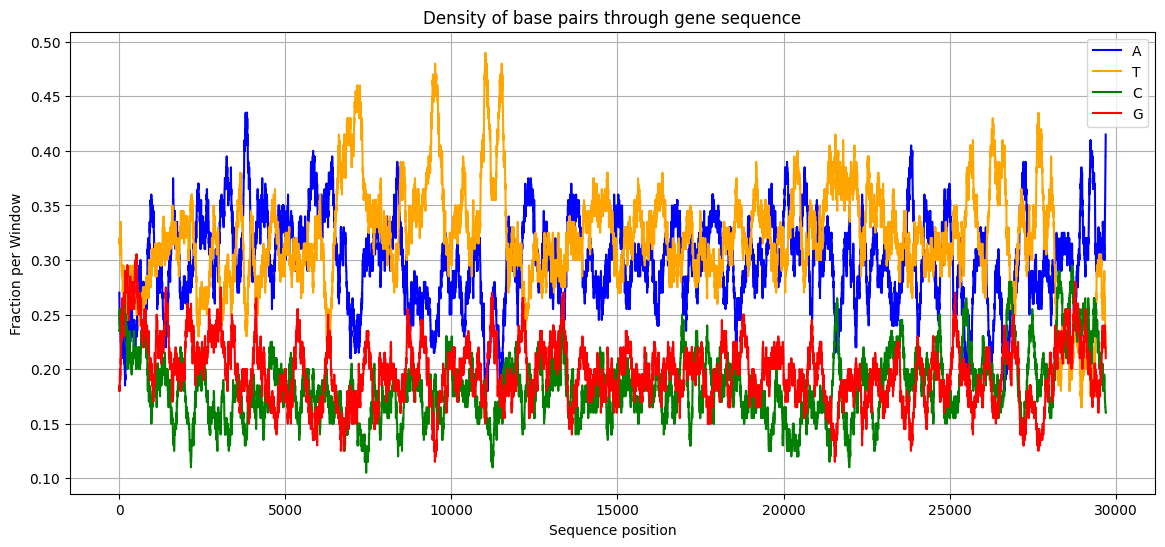
\includegraphics[width=\textwidth]{../code/density.png}
        \caption{Density of Base Pairs in SARS-CoV-2}
        \label{fig:density}
    \end{subfigure}
    \hfill
    % Second Subfigure (Top Right)
    \begin{subfigure}[t]{0.45\textwidth}
        \centering
        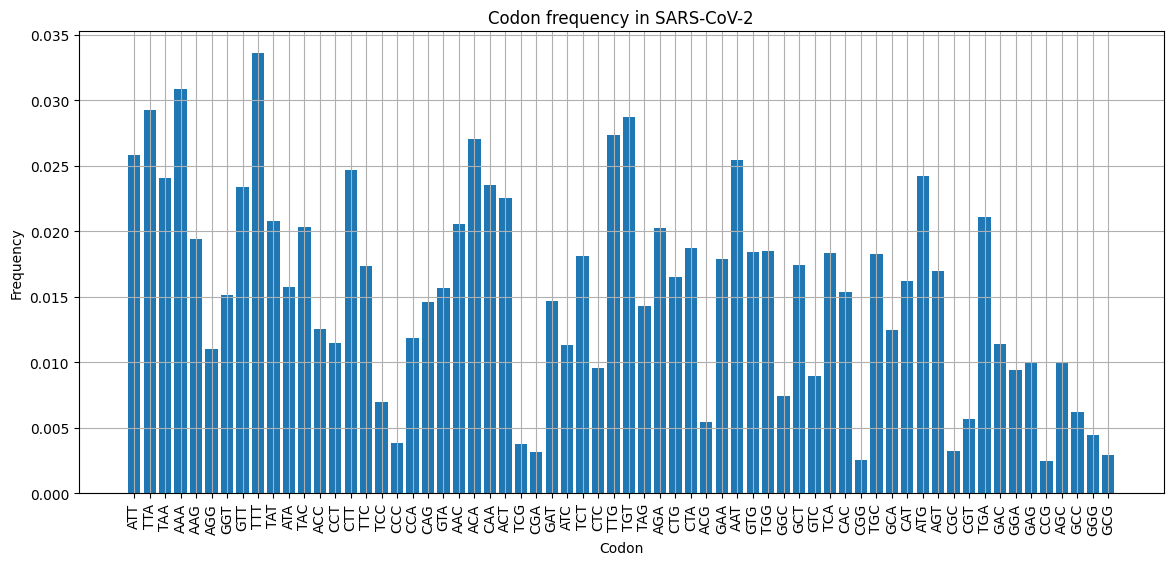
\includegraphics[width=\textwidth]{../code/histoSC2.png}
        \caption{Codon Frequency in SARS-CoV-2}
        \label{fig:histosc2}
    \end{subfigure}

    \vspace{1em}  % Space between rows

    % Third Subfigure (Bottom Left)
    \begin{subfigure}[t]{0.45\textwidth}
        \centering
        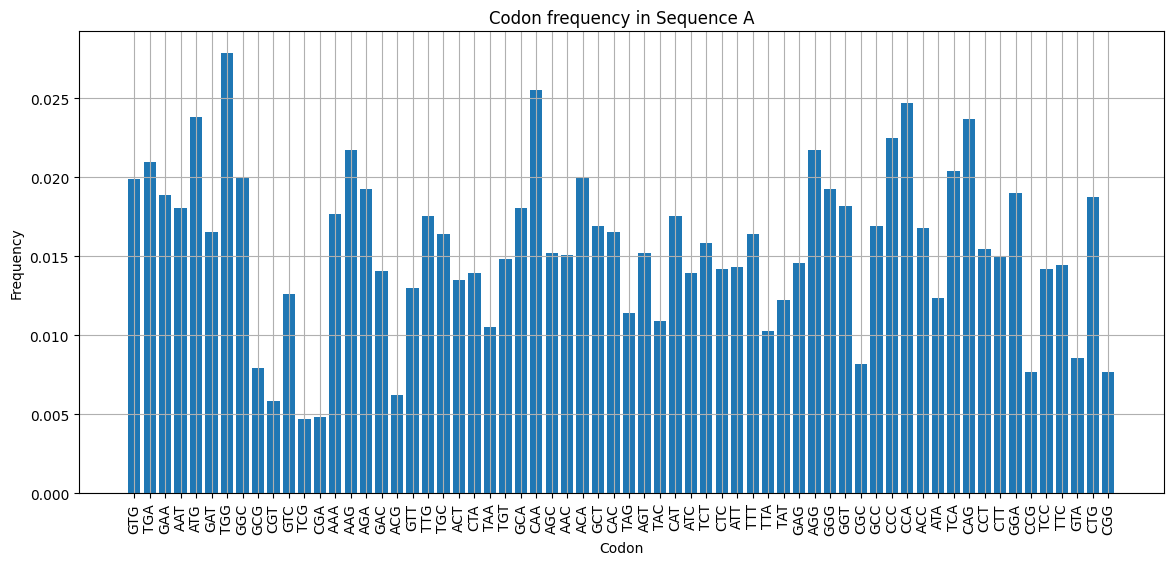
\includegraphics[width=\textwidth]{../code/histoA.png}
        \caption{Codon Frequency in Gene Sequence A}
        \label{fig:histob}
    \end{subfigure}
    \hfill
    % Fourth Subfigure (Bottom Right)
    \begin{subfigure}[t]{0.45\textwidth}
        \centering
        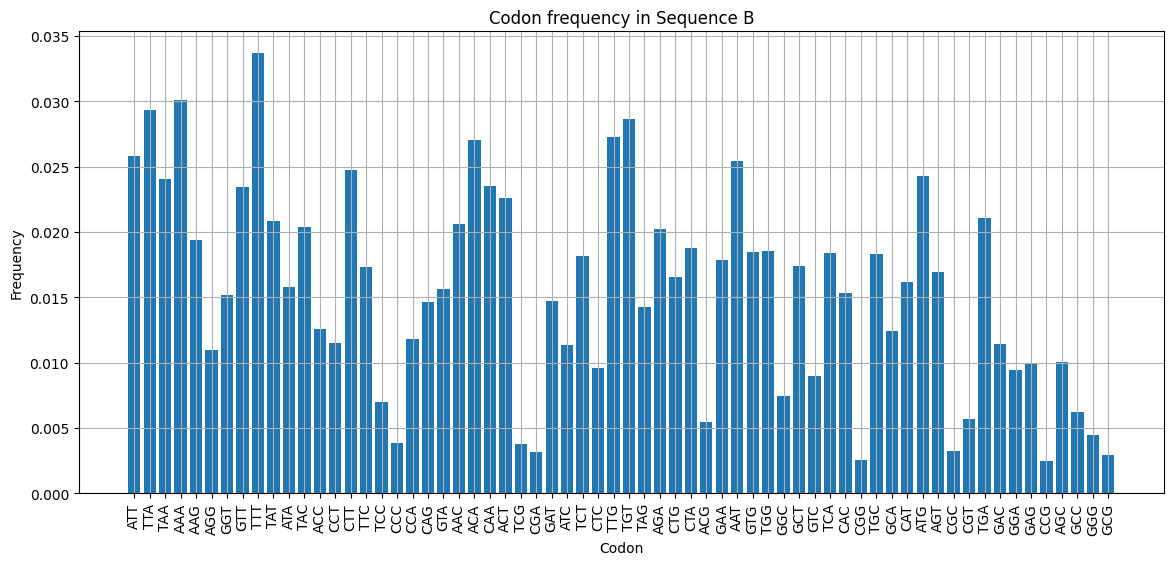
\includegraphics[width=\textwidth]{../code/histoB.png}
        \caption{Codon Frequency in Gene Sequence B}
        \label{fig:histoa}
    \end{subfigure}

    \label{fig:all_figures}
\end{figure}
% of LLM output

\subsection*{2.}
Kullback-Leibler values between:\\
Sequence A and SARS-CoV-2: \num{0.1380117294430006}\\
Sequence B and SARS-CoV-2: \num{9.028641025468603e-06}

\subsection*{3.}
it is most likely that Sequence B is a covid variant you can see this by observation in comparing
figure 1b with figure 1d. It can also be seen quantitatively by see how much smaller the Kullback-Leibler value of 
Sequence B when compared to SARS-CoV-2 

\subsection*{4.}
if were were to use count to find the count of all the unique codons we would have to iterate through all the 
possible codons. the dictionary method is much better, just inching along the gene and every time you check the codon
and dictionaries have very nice tools to tell if and how many of them have been found.

\subsection*{5.}
\begin{figure}[h]
    \centering
    % First Subfigure (Top Left)
    \begin{subfigure}[t]{0.45\textwidth}
        \centering
        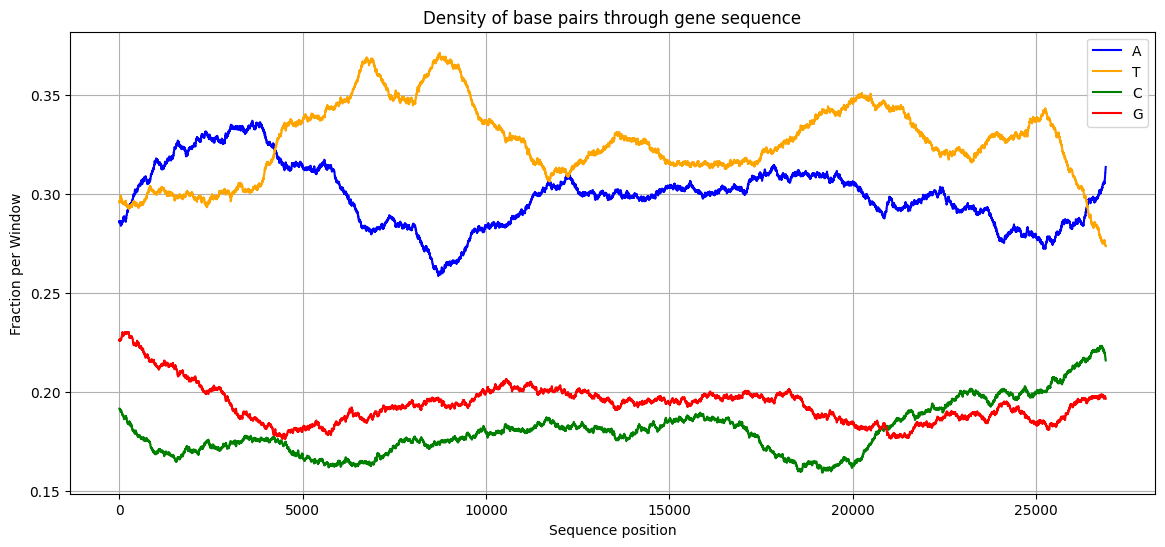
\includegraphics[width=\textwidth]{density3000nwind.png}
        \caption{High nWind of 3000}
        \label{fig:density}
    \end{subfigure}
    \hfill
    % Second Subfigure (Top Right)
    \begin{subfigure}[t]{0.45\textwidth}
        \centering
        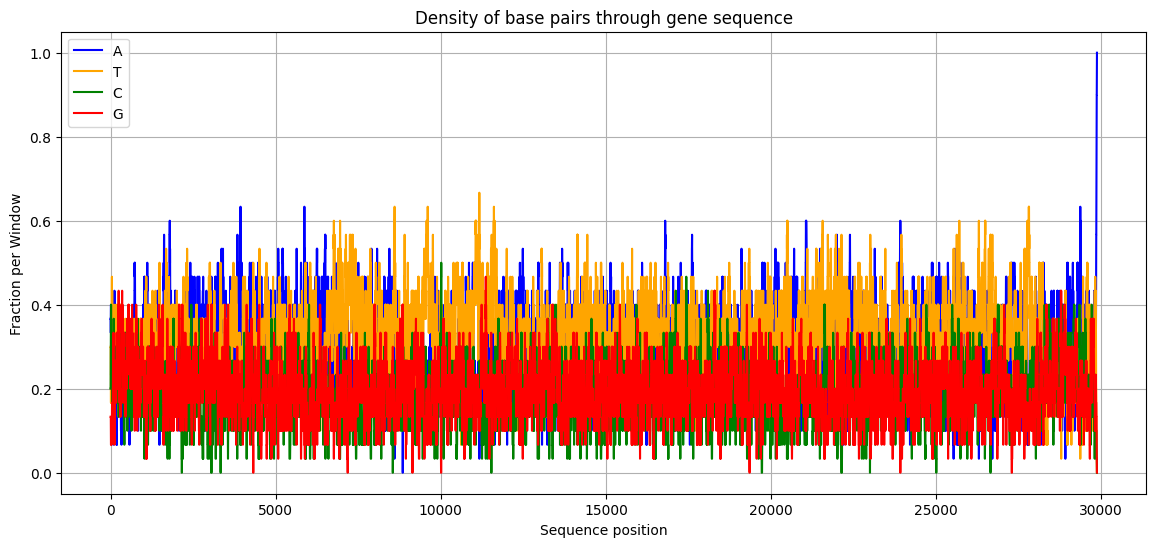
\includegraphics[width=\textwidth]{density30nwind.png}
        \caption{Low nWind of 30}
        \label{fig:histosc2}
    \end{subfigure}
\end{figure} 
from the figures you can see that a higher n window gives a higher correlation between A and T base pairs
as well as between C and G base pairs which makes sense cause they are sister pairs.

\end{document}
